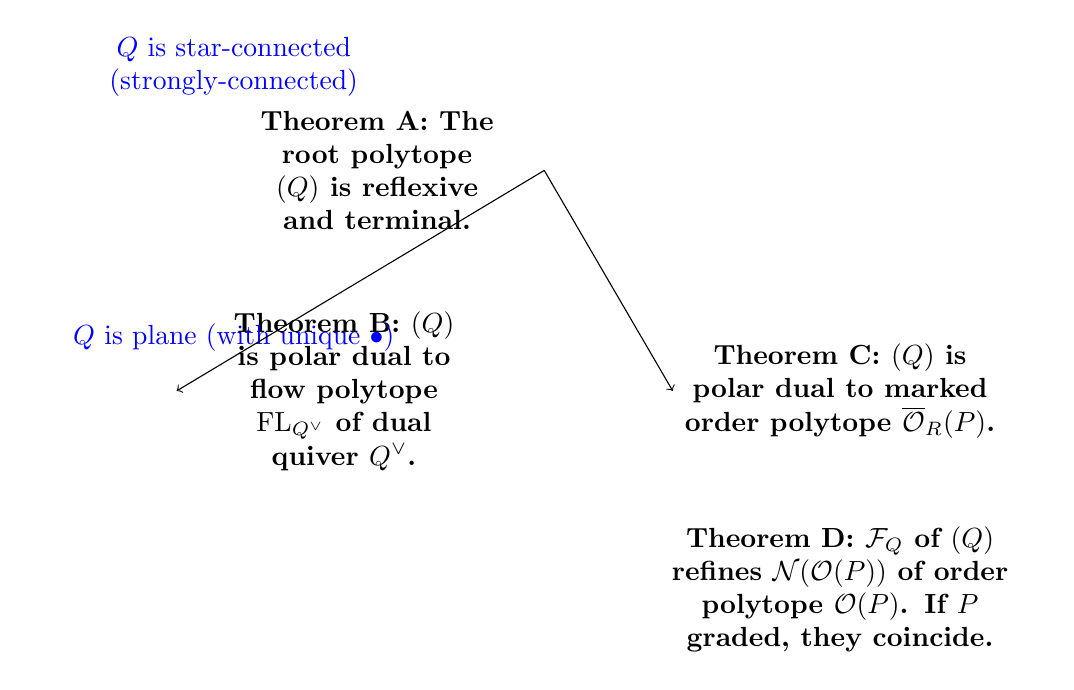
\begin{tikzpicture}[scale=1.4]
\node[align=center,font=\bfseries,text width=4cm] (A) at (-4.7,0) {Theorem A: The root polytope $\Root(Q)$ is reflexive\\and terminal.};
\node[align=center,text width=5cm,anchor=north,text=blue] (B) at (-6,1.3) {$Q$ is star-connected (strongly-connected)};
\node[align=center,font=\bfseries,text width=4cm] (C) at (-5,-2) {Theorem B: $\Root(Q)$ is polar dual to flow polytope \\${\rm FL}_{Q^\vee}$ of dual quiver $Q^\vee$.};
\node[align=center,text width=5cm,anchor=north,text=blue] (D) at (-6,-1.3) {$Q$ is plane (with unique $\bullet$)};
\node[align=center,font=\bfseries,text width=4cm] (E) at (-0.5,-2) {Theorem C: $\Root(Q)$ is polar dual to marked order polytope ${\overline{{\mathcal O}}}_R(P)$.};
\node[align=center,font=\bfseries,text width=5cm] (F) at (-0.5,-3.8) {Theorem D: ${\mathcal F}_Q$ of $\Root(Q)$ refines ${\mathcal N}({\mathcal O}(P))$ of order polytope ${\mathcal O}(P)$. If $P$ graded, they coincide.};
\draw [->] (A.east) -- (C.west);
\draw [->] (A.east) -- (E.west);
\end{tikzpicture}